\message{ !name(GTproblem.tex)}
\message{ !name(GTproblem.tex) !offset(-2) }
The Gear Train design problem is a classic multi-objective optimization
problem, for it encompasses a number of the challenges that a practical
real-world optimization task may present. It involves a number of variables
of different types and a large number of equality and inequality
constraints. A number of conflicting objectives can be considered for the
optimization. This problem was analyzed in \cite{agogino1990} to explain
the design process from an optimization perspective, and in \cite{debgt} to
prove the applicability of NSGA-II in complex optimization tasks. We
analyze the pareto-optimal solutions of this design-optimization problem to
discover chunks of optimal designs using our proposed procedure.


\section{Problem description}
\label{problem}
The objective of multi-speed gearbox design is to obtain different
specified speeds in the output shaft with fixed input shaft angular
velocity. The two-dimensional layout of a 18-speed gearbox with 18 gears is
shown in figure \ref{geartrain}. Gears in shafts 1, 3 and 5 can be
translated to mesh with corrsponding gears in shafts 2, 4 and 6 to obtain
desired output speed. The input shaft speed is kept fixed at 1400 rpm. With
a ratio of 1.14 between consecutive output speeds, the $i^{th}$ desired
output speed would be $1400/(1.14)^{i-1}$.  The lowest desired speed is
thus $1400/(1.14)^{17} = 150$ rpm.

\begin{figure}[ht]\begin{center}
 \fbox{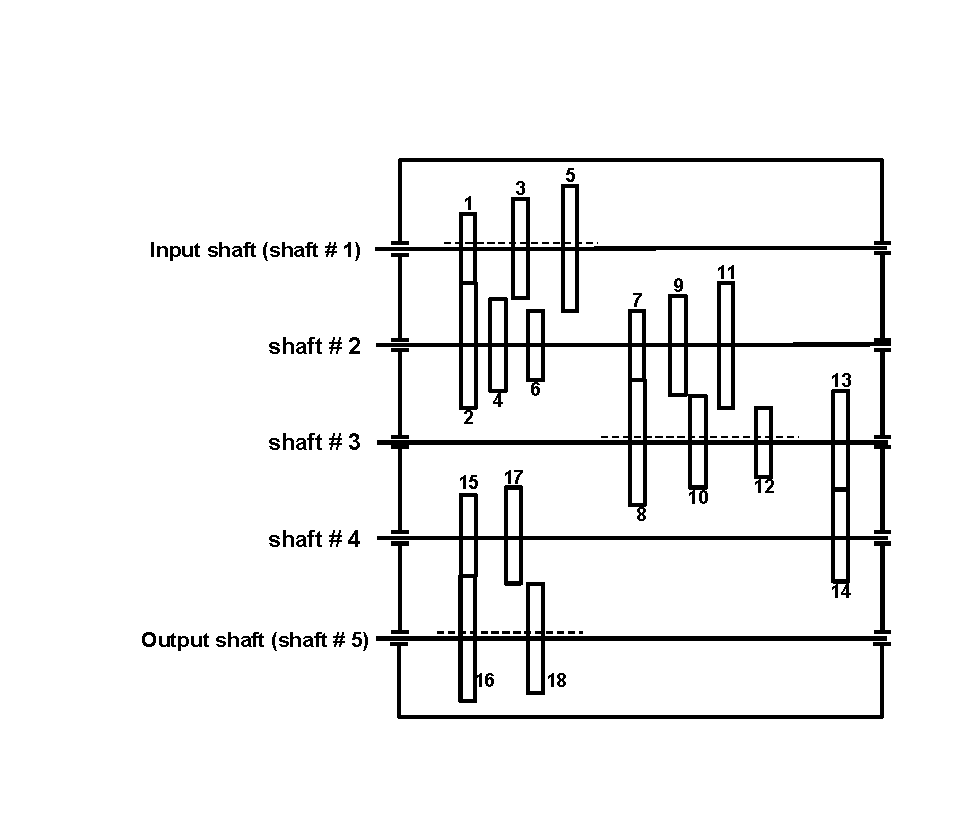
\includegraphics[width=100mm, height=80mm]{diagrams/geartrain.eps}}
 \caption{18-speed Gear-train schematics}
 \label{geartrain}
\end{center}\end{figure}

A number of objectives can be considered for the design of the gear 
train design optimization, e.g.:

\begin{enumerate}[(i)]
\item minimization of the gear material used,
\item maximization of the power delivered, 
\item minimization of the centre distance between input and output 
shaft,
\item minimization of the error between desired and achieved output 
speeds.
\end{enumerate}

There are a large number of design parameters on which the optimization
problem can be defined, depending on the aspects of the design we want to
explore. Here we will consider two instances of the problem, one in which
all the thickness of all the gear-pairs and gear-module thickness is
varied, and one in which number of teath in all the gears in addition to
gear-pair thickness and gear-module thickness is varied. For the first case
we will fix the number of teeth in each gear and consider two obejectives
(maximize power delivered, and minimize gear material), and for the second
case number of teeth in all the gears are variable and one extra objective
(minimization of maximum error in output speeds) will be considered.  There
are 11 design variables for the first case, and 29 variables for the
second.

\subsection{Multi-objective optimization formulation for the 
11-parameters design problem}

The eleven variables for the first optimization scenario we are going 
to consider are:

\begin{enumerate}[(i)]
\item thickness of gear-paris, $t_i$ for $i = 1, 2, \dots G$
\item teeth module, the same for all the gear pairs, and
\item the power delivered $p$
\end{enumerate}

We take two conflicting objectives for this design simulation-- 
maximizing the power delivered, $f_1$ and minimizing the total volume
of gear material used, $f_2$. The complete optimization problem is 
given as follows:

\begin{singlespacing}
\begin{flushleft}


\begin{align}
\text{Maximize} \quad f_1 &=     \left. p,       \right.\nonumber\\
\text{Minimize} \quad f_2 &= \left. \frac{\pi m^2}{4} {\displaystyle\sum\limits_{i=1}^G {({n^2_{p_i}} + {n^2_{w_i}}) t_i }}\right.\nonumber\\
\text{Subject to,} \qquad & \left. \right.\nonumber\\
{\sigma}_{b_i} &\leqslant  S_b \quad  &\left. \text{for} \quad i = 1, 2, \dots G, \right.\nonumber\\
{\sigma}_{w_i} &\leqslant S_w \quad   &\left. \text{for} \quad i = 1, 2, \dots G, \right.\nonumber\\
t^{(L)} &\leqslant t_i \leqslant t^{(U)}   &\left. \text{for} \quad i = 1, 2, \dots G, \right.\nonumber\\
p^{(L)} &\leqslant p \leqslant p^{(U)} 
\end{align}

Where, 

\end{flushleft}

\begin{itemize}
\item $m$ is the teeth module for all the gear pairs,
\item $n_{p_i}$ and $n_{w_i}$ are the number of teeth in the pinion 
and wheel in the $i^{th}$ gear-pair,
\item $t_i$ is the thickness of the gear-pair in cm., 
\item ${\sigma}_{b_i}$ is the bending stress developed in a gear-pair 
calculated as follows:

\begin{equation}
\sigma_{b_{i}} = \frac{97500 p { } k_c { } k_d { } (r_i + 1)} {a_{ i} { } {\omega}_{ i} { } t_{ i} { } m { } r_{ i} { } y_{ i} { } \text{cos} \beta} \\
\end{equation}

\item $S_b$ ($= 2,500\text{ kgf}/\text{cm}^2$) is the permissible bending stress,

\item ${\sigma}_{w_i}$ is the wearing stress developed in a gear-pair
calculated as follows:

\begin{equation}
\sigma_{w_{i}} = \frac{o.59 (r_i+1)}{r_i a_i} \sqrt{\frac{97500 p { } k_c { } k_d { } E (r_i + 1)}{ {\omega}_i t_i \text{sin} 2 \beta}}
\end{equation}
\item $S_w$ ($= 17,500\text{ kgf}/\text{cm}^2$) is the permissible wearing stress,

\item $k_c(=1.5)$ is the stress concentration factor,
\item $k_d(=1.1)$ is the dynamic load factor,
\item $r_i$ is the transmission ratio, defined as the ratio of number 
of teeth in the wheel $(n_{w_i})$ to the number of teeth in the 
pinion $(n_{p_i})$ for the $i^{th}$ gear-pair,
\item ${\omega}_i$ is the angular velocity of the wheel in rpm,
\item $a_i$ is the centre distance for the corresponding gear pair
given as 
\\
$a_i = \frac {m ( n_{w_i} + n_{p_i})} {2}$ , 
\item $y_i$ is the form load factor defined as 
$y_i = 0.52(1+ \frac{20}{n_{w_i}} )$ , 
\item ${\beta}(= 20 \text{ degrees})$ is the pressure angle,
\item $E $ ($= 2.1 \times 10^6\text{ kgf}/\text{cm}^2$) is the Young's modulus of the gear material. .
\end{itemize}

\end{singlespacing}


\subsection{Extending to 29 design variables}
To have varying number of teeth in the gears, the following 
constraints must be satisfied by all feasible gear-train designs:

\begin{enumerate}
\item All mating gear-pairs on  two shasfts should have the same 
centre distances as the shaft distances.
\item Since we have a two-dimensional gear-train layout, no gear 
should interfere with any shaft.
\item Maximum gear ratio in any gear pair should not exceed a limit 
$r^{max}$.
\end{enumerate}

The overall optimization problem formulation is the same as given is the 
same as given in the previous subsection, except we have 18 new 
variables in the form of number of gear teeth, $n_i$ (for $i = 1, 2,
\dots G$), and the above discussed constraints. The above constraints
are formulated as follows:


\begin{singlespacing}
\begin{flushleft}

{\allowdisplaybreaks
\begin{align}
& n_1 + n_2 = n_3 + n_4 = n_5 + n_6,  \quad &\left. \text{(between shaft 1 and 2)} \right.\nonumber\\
& n_7 + n_8 = n_9 + n_{10} = n_{11} + n_{12}, \quad &\left. \text{(between shaft 2 and 3)} \right.\nonumber\\
& n_{15} + n_{16} = n_{17} + n_{18} \quad &\left. \text{(between shaft 4 and 5)} \right.\\
\nonumber\\
&n_2 \leqslant n_7 + n_8, \quad n_4 \leqslant n_7 + n_8, \nonumber\\
&n_6 \leqslant n_7 + n_8, \quad n_7 \leqslant n_1 + n_2, \\
\nonumber\\
&n_9 \leqslant n_1 + n_2, \quad n_{11} \leqslant n_1 + n_2, \nonumber\\
&n_8 \leqslant n_{13} + n_{14}, \quad n_{10} \leqslant n_{13} + n_{14},\\
\nonumber\\
&n_{12} \leqslant n_{13} + n_{14}, \quad n_{13} \leqslant n_7 + n_8, \nonumber\\
&n_{14} \leqslant n_{15} + n_{16}, \quad n_{15} \leqslant n_{13} + n_{14},\\
\nonumber\\
& n_{17} \leqslant n_{13} + n_{14}\\
\nonumber\\
& | {\Omega}_k - {\Omega}^I_k | \leqslant \epsilon {\Omega}^I_k\\
\nonumber\\
& \frac{n_{w_i}} {n_{p_i}}  \leqslant r^{max} \quad &\left. \text{(for i = 1, 2, \dots G)} \right.\nonumber\\
& n_{w_i} \geqslant n^{(L)} &\left. \text{(for i = 1, 2, \dots G)} \right.\nonumber\\
& n_{p_i} \geqslant n^{(L)} &\left. \text{(for i = 1, 2, \dots G)} \right.\nonumber\\
& n_i \in \mathbb{Z} &\left. \text{(for i = 1, 2, \dots 2G)} \right.
\end{align}
}
\end{flushleft}
\end{singlespacing}

\subsection{NSGA-II formulation and the pareto-front}
We use the same NSGA-II formulation as in \cite{debgt} to obtain the
pareto-optimal solutions. For the 11 variables case we fix the 
gear-box layout by fixing the number of teeth in each gear to the 
values shown in table \ref{gearTeeth}. 

\begin{table}[!ht]
\centering
\begin{tabular}{c|c|c|c|c|c|c|c|c|c|}
\cline{2-10}
& 1 & 2 & 3 & 4 & 5 & 6 & 7 & 8 & 9  \\
\hline
\multicolumn{1}{|c|}{$n_{p_i}$} & 20 & 33 & 28 & 32 & 34 & 33 & 33 & 20 & 26\\
\hline
\multicolumn{1}{|c|}{$n_{w_i}$} & 56 & 43 & 48 & 37 & 35 & 36 & 34 & 54 & 48\\
\hline
\end{tabular}
\caption{No. of teeth for each gear-pair in fixed layout gear-train design}
\label{gearTeeth}
\end{table}

In second case we utilize the equality constraints given in equations 3.4
to eliminate five gear teeth variables. We code the gear teeth variables in
such a way so as to avoid evaluating permutations of same combinations of
gears in each transmission stage. Also, we condense similar constraints
into one constraint wherever possible. The probabilities of recombination
and mutation operator are 0.9 and 0.3 respectively for both the
optimization cases. For the 11 variables optimization, we run NSGA-II for
600 generations with a population size of 3000, and for 10000 generations
with 3000 initial population for the 29 variable case. NSGA-II yeilds 927
points in the pareto-front for the first case. The pareto-front for the 29
variables optimization has 422 points. The pareto-fronts are shown in
figures \ref{gt11Clusters} and \ref{gtvClusters}.


\section{Recovering chunks in the pareto-front}

\subsection{The fixed lay-out problem}
Figure \ref{gt11rv} shows the Isomap residual variances for the
pareto-front of the fixed gear-box lay-out pareto-front. The largest drop
in the Isomap residual variance from 3 to 4 dimensional Isomap
embedding. This implies that the pareto-front has an intrinsic
dimensionality of four, and we can expect to have clusters of dimensions
lower than 4.

The PCA explained variance is shown in \ref{gt11ev}, which clearly shows
that the pareto-front is one dimensional in the parameter space. Table
\ref{first2GTPCs} shows the weights of five variables which have the
highest absolute component in in the first two principal components. The
thicknesses of the gear pairs in the final transmission stage are the
variables with the highest weightage in the first principal component. Next
are the thickness of the second and fifth gear-pairs. In the second
principal component, the gear module is the most important
variable. Weights of all the other variables are  negligible in this
principal component.


% \begin{figure}[ht]\begin{center}
%  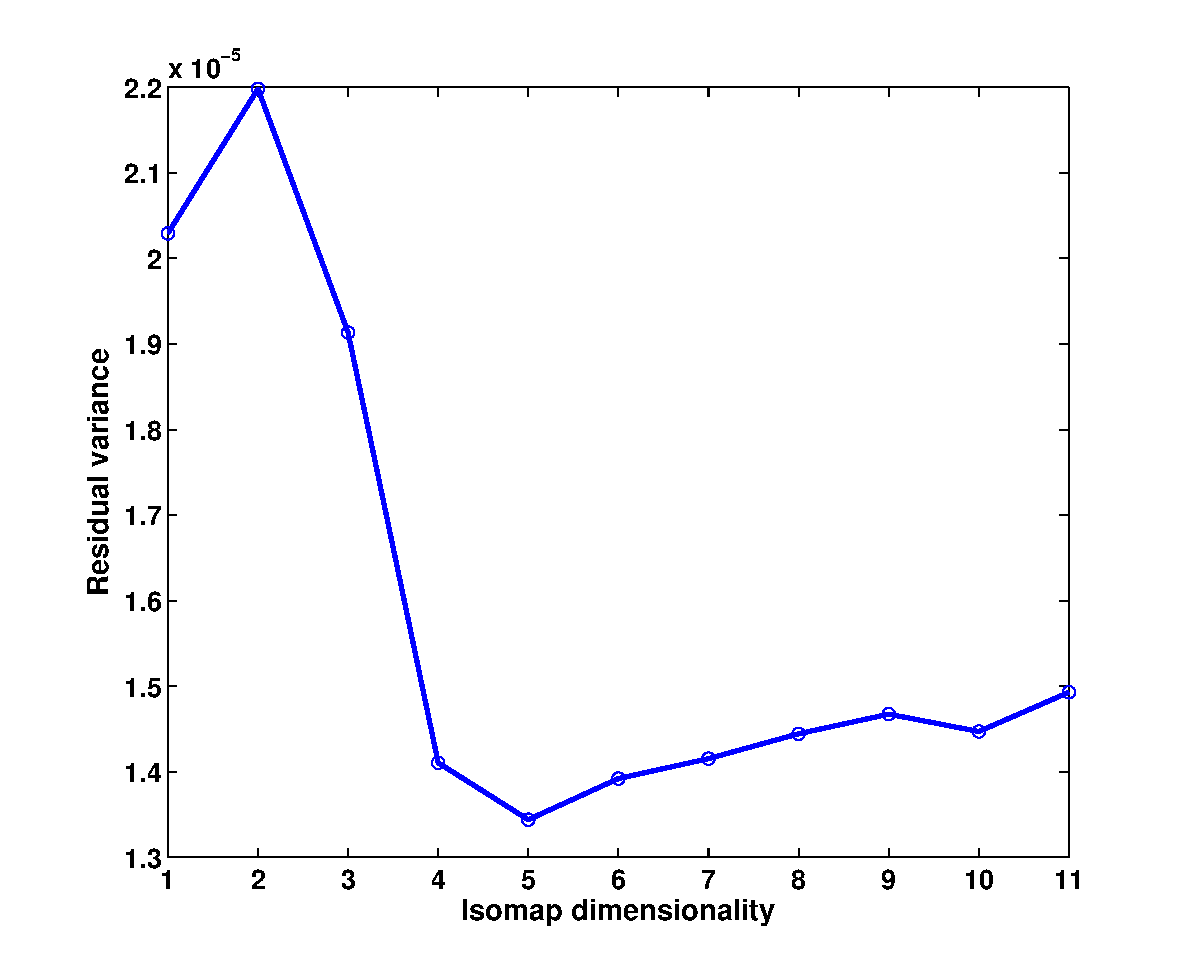
\includegraphics[width=100mm, height=80mm]{dia/gt11rv.eps}
%  \caption{Isomap residual variance for the fixed lay-out paret-front}
%  \label{gt11rv}
% \end{center}\end{figure}

\begin{figure}[ht]\begin{center}
 \subfloat[Isomap Residual Variance]{
 \label{gt11rv} 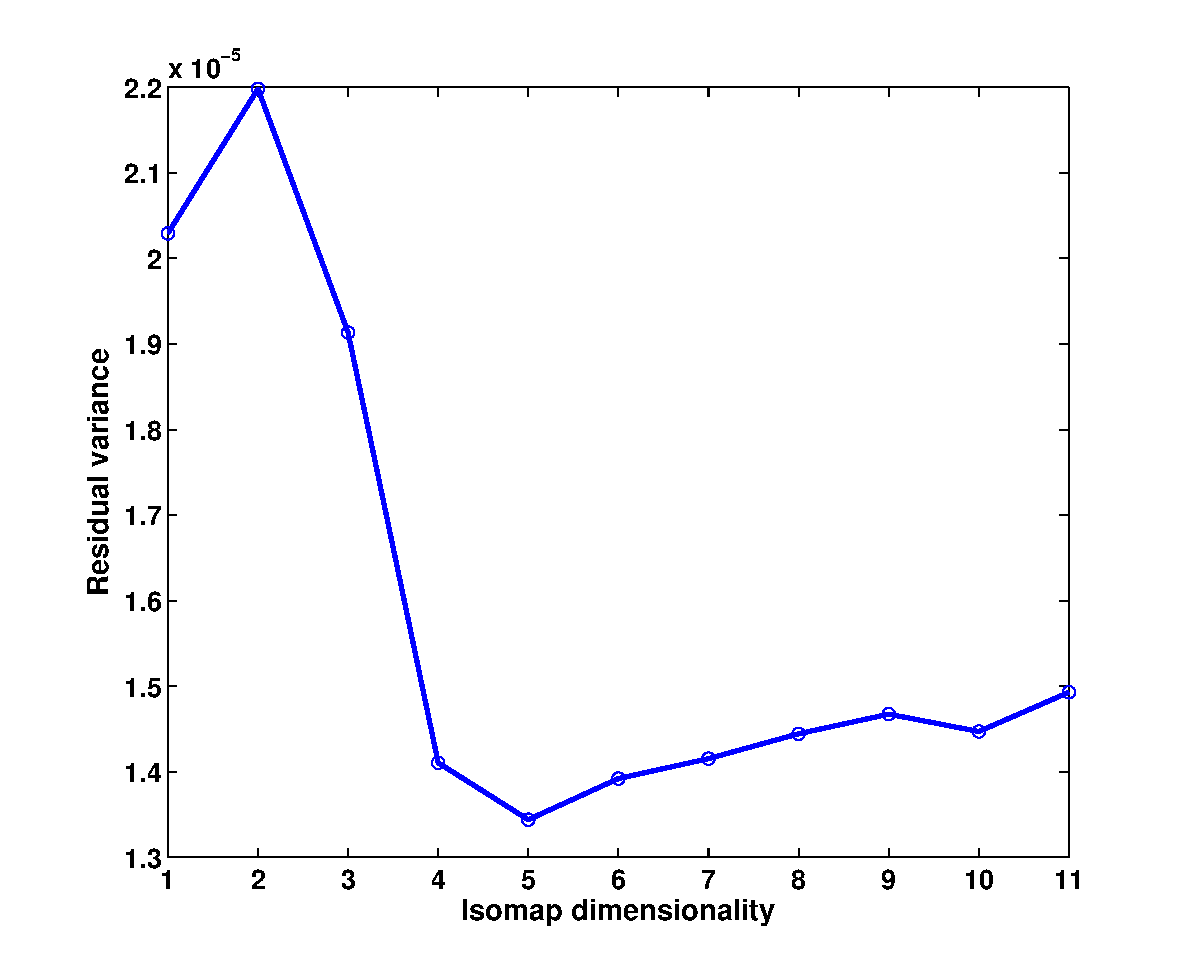
\includegraphics[width=62mm, height=52mm]{dia/gt11rv.eps}}
 \subfloat[PCA Explained variance]{
 \label{gt11ev} 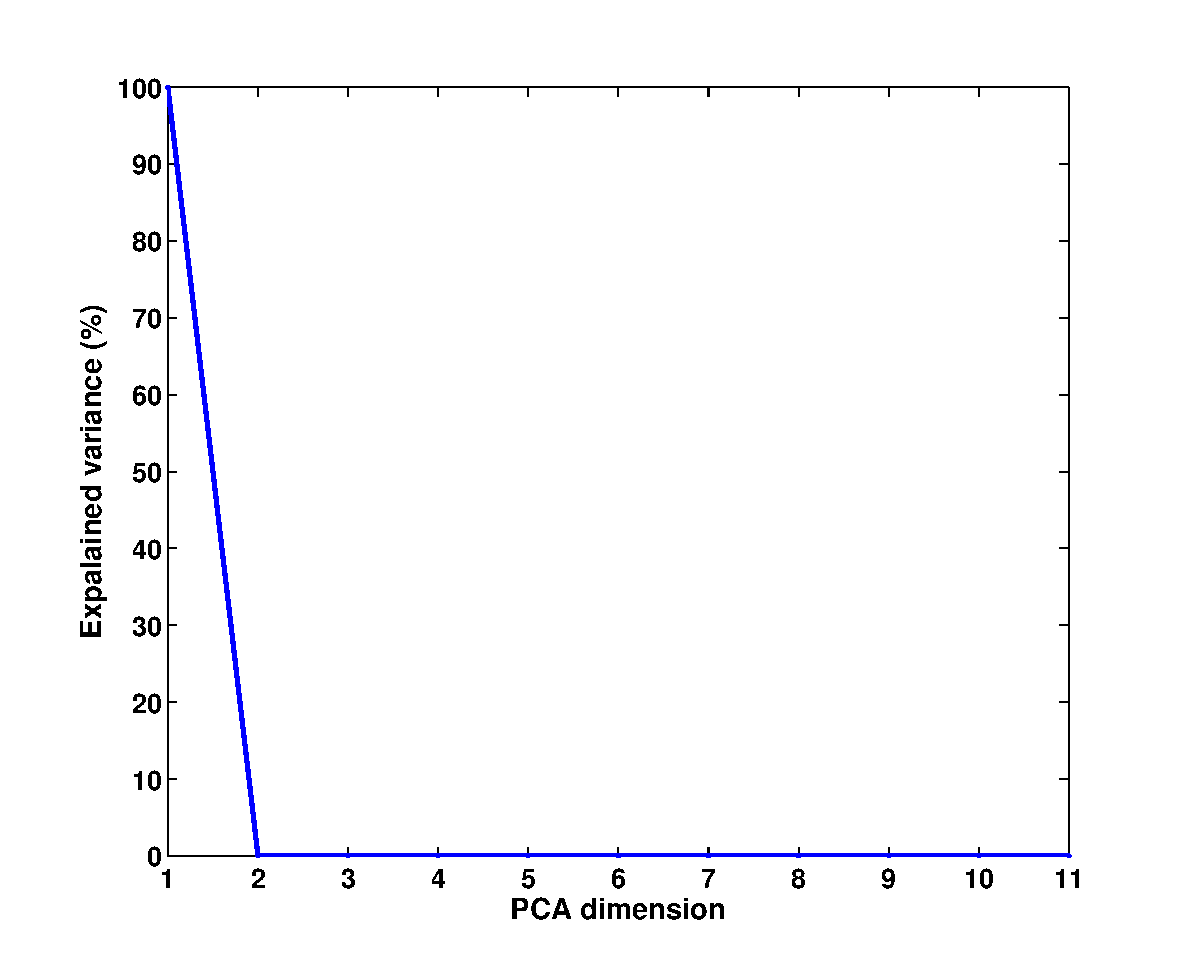
\includegraphics[width=62mm, height=52mm]{dia/gt11ev.eps}}
 \caption{Isomap and PCA results for the fixed lay-out problem}
 \label{gt11Var}
\end{center}\end{figure}

\begin{table}[!ht]
  \centering
  \begin{tabular}{|c|c|c|c|c|c|}
    \hline
    \multirow{2}{*}{First PC}   & ($t_9$) &  ($t_8$) &  ($t_7$)  & ($t_6$) & ($p$)\\
    & -0.8444  & -0.4617  & 0.1837 & -0.1511 & 0.0733  \\
    \hline
    \multirow{2}{*}{Second PC}   & ($m$) &  ($t_5$) &  ($t_6$)  & ($t_9$) & ($t_8$)\\
    & 0.9997 & -0.0124 & 0.0097 & 0.0087 &  0.0087 \\
    \hline
  \end{tabular}
  \caption{First two principal components of the BDCPM data}
  \label{first2GTPCs}
\end{table}

\subsubsection{Clusters in the pareto-front}
Although it is possible to cluster the pareto-front into smaller clusters by varying the 
$k$ paramenter in our clustering algorithm, we show and analyze significantly sized and 
smaller number of clusters for the sake of simplicity. Figure \ref{gt11clusters} shows 
the 11 clusters obtained by setting $k = 6.0$.


\begin{figure}[ht]\begin{center}
 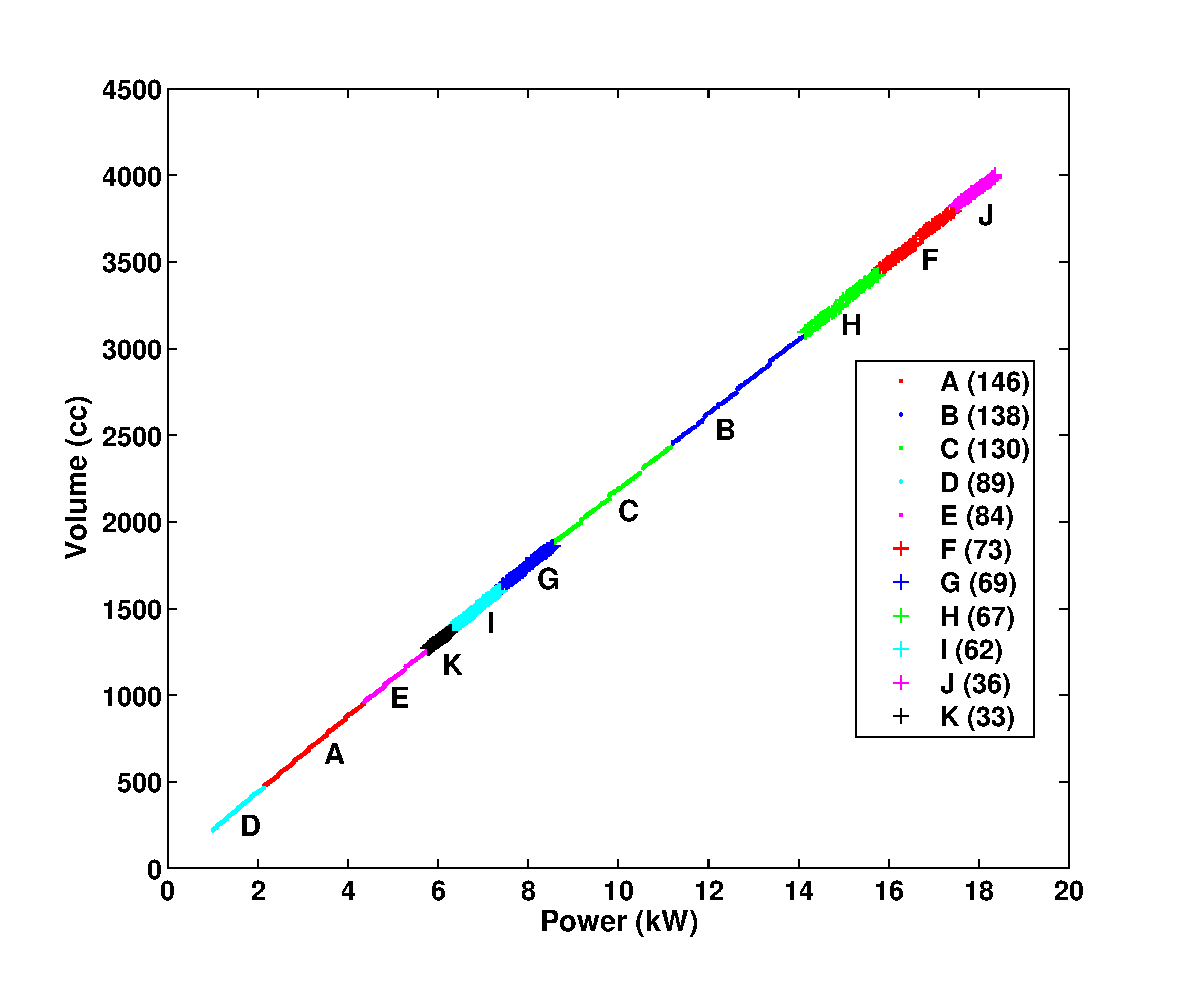
\includegraphics[width=100mm, height=80mm]{dia/gt11cpareto1.eps}
 \caption{Clusters for the 11-variable problem}
 \label{gt11Clusters}
\end{center}\end{figure}

% \begin{figure}[ht]\begin{center}
%  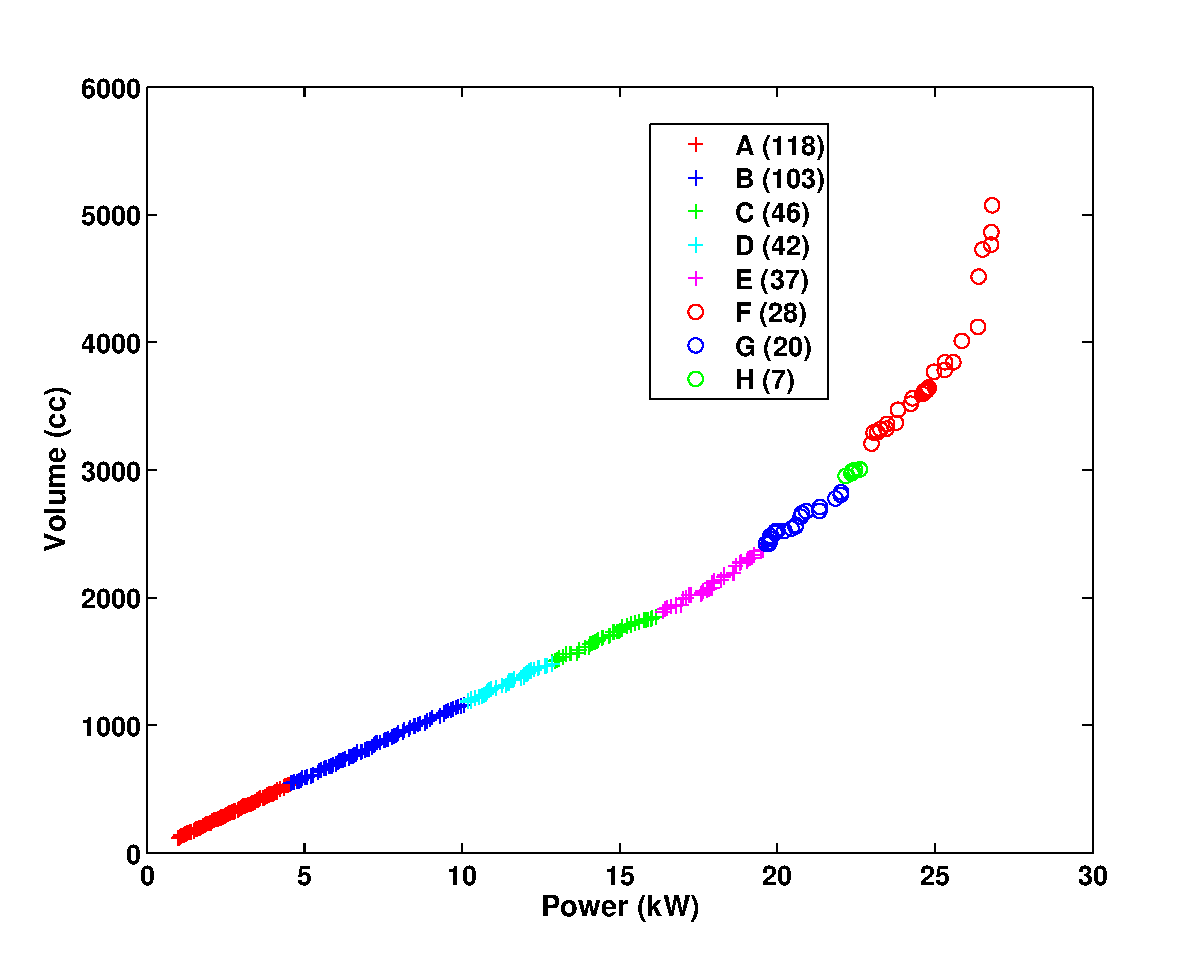
\includegraphics[width=100mm, height=80mm]{dia/gt29clusters.eps}
%  \caption{Clusters for the 29-variable problem}
%  \label{gt29clusters}
% \end{center}\end{figure}




\begin{figure}[ht]\begin{center}
 \subfloat[Isomap Residual Variance for the cluster D]{
 \label{gt11rv} 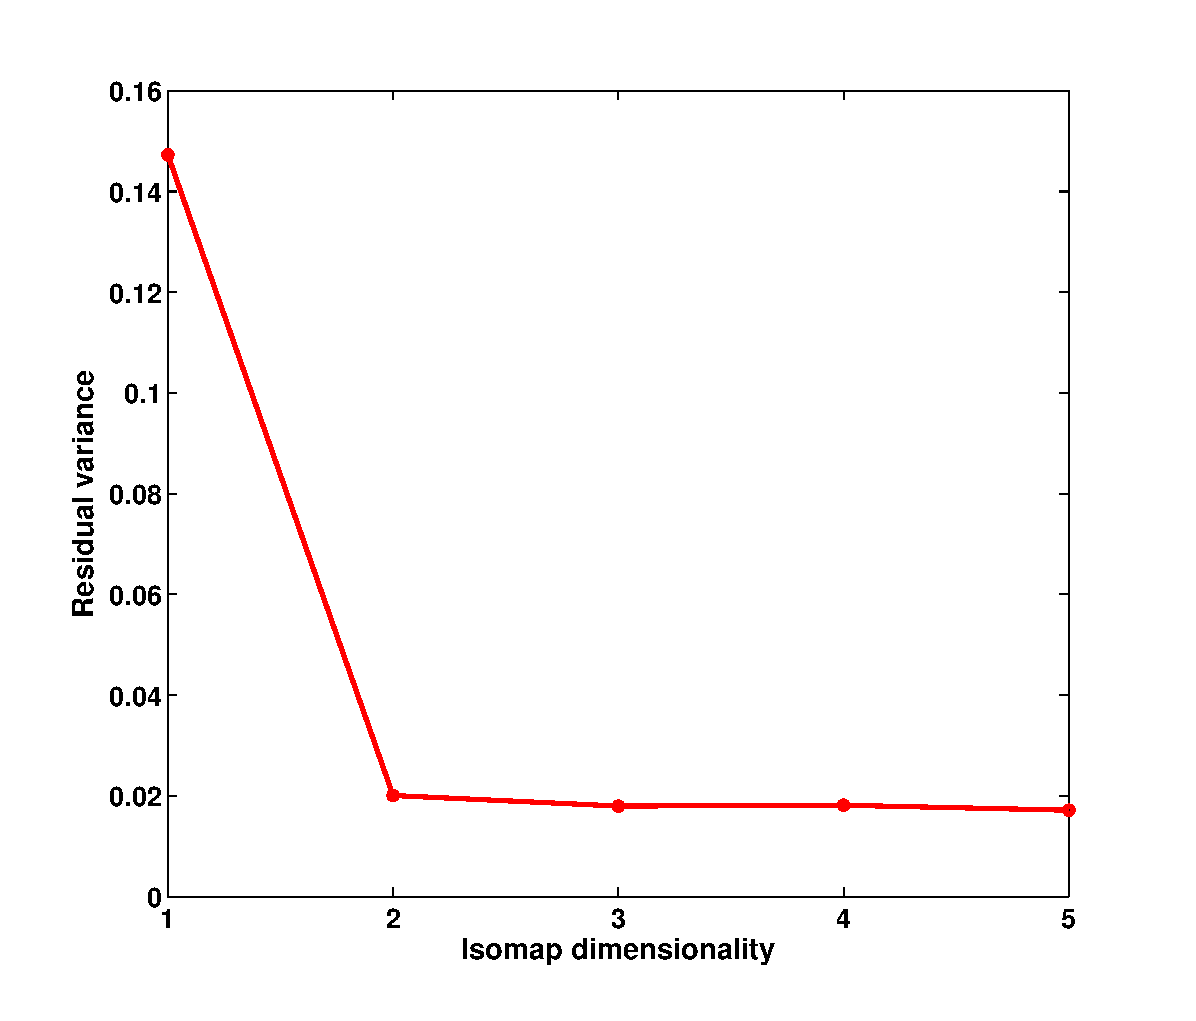
\includegraphics[width=62mm, height=52mm]{dia/gt11cluster4rv.eps}}
 \subfloat[PCA Explained variance for some clusters having explained variance of more than 1\% for second principal component]{
 \label{gt11ev} 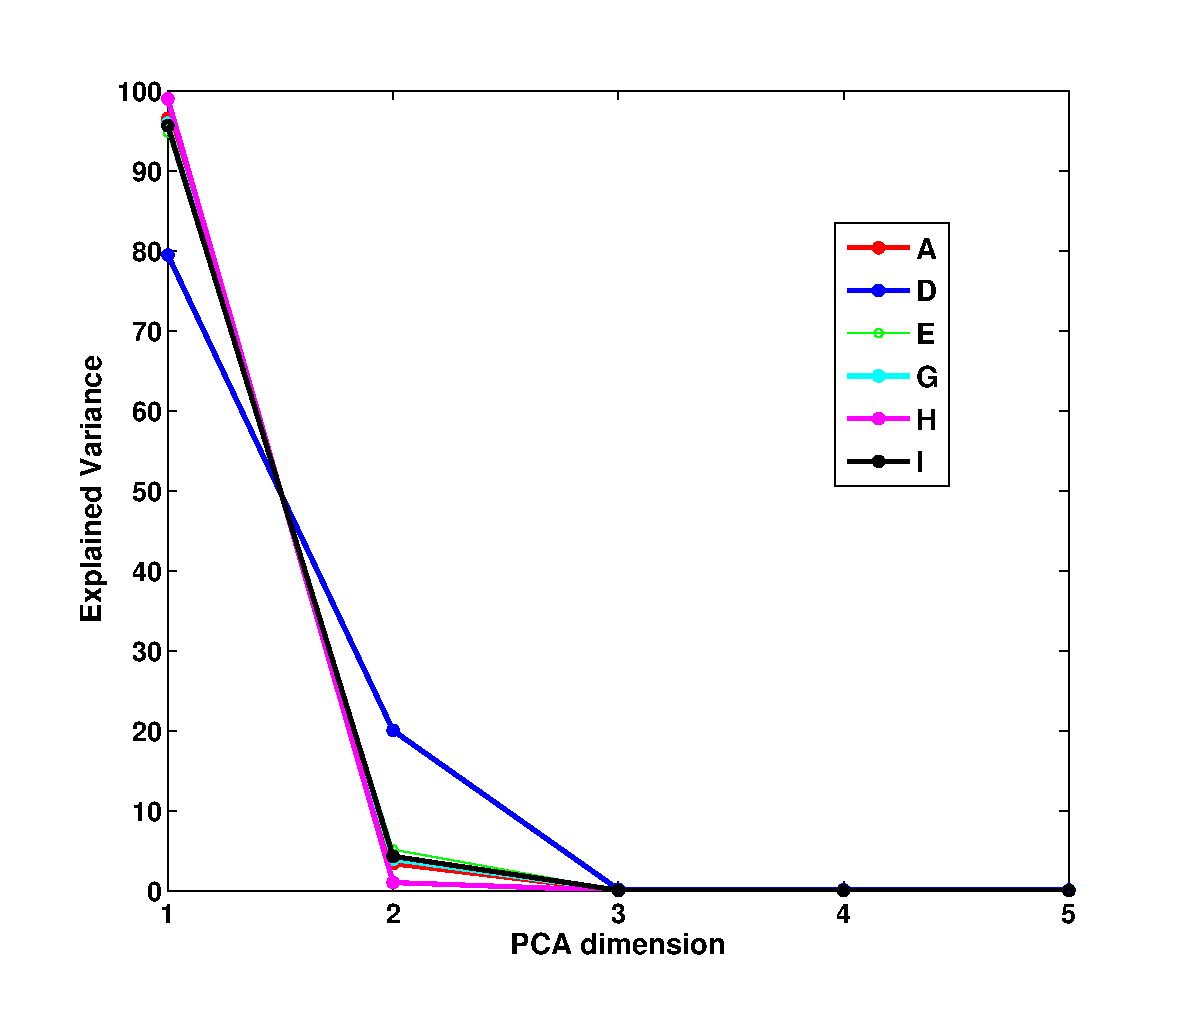
\includegraphics[width=62mm, height=52mm]{dia/gt11clustersEV.eps}}
 \caption{Isomap and PCA results for the clusters of fixed lay-out problem}
 \label{gt11clustersVar}
\end{center}\end{figure}


\begin{table}[!ht]
  \centering
  \begin{tabular}{|c|c|c|c|c|c|c|}
    \hline
    Gear pair No. & 1 & 8 & 9 & 2 & 4 & 5 \\
    \hline
    I/O Speed ratio & 0.357 & 0.464 & 0.541 & 0.767 & 0.864 & 0.970 \\
    \hline
  \end{tabular}
  \caption{Gear pairs with lowest input to output speed ratios.}
  \label{iosRatio}
\end{table}


\begin{figure}[ht]\begin{center}
 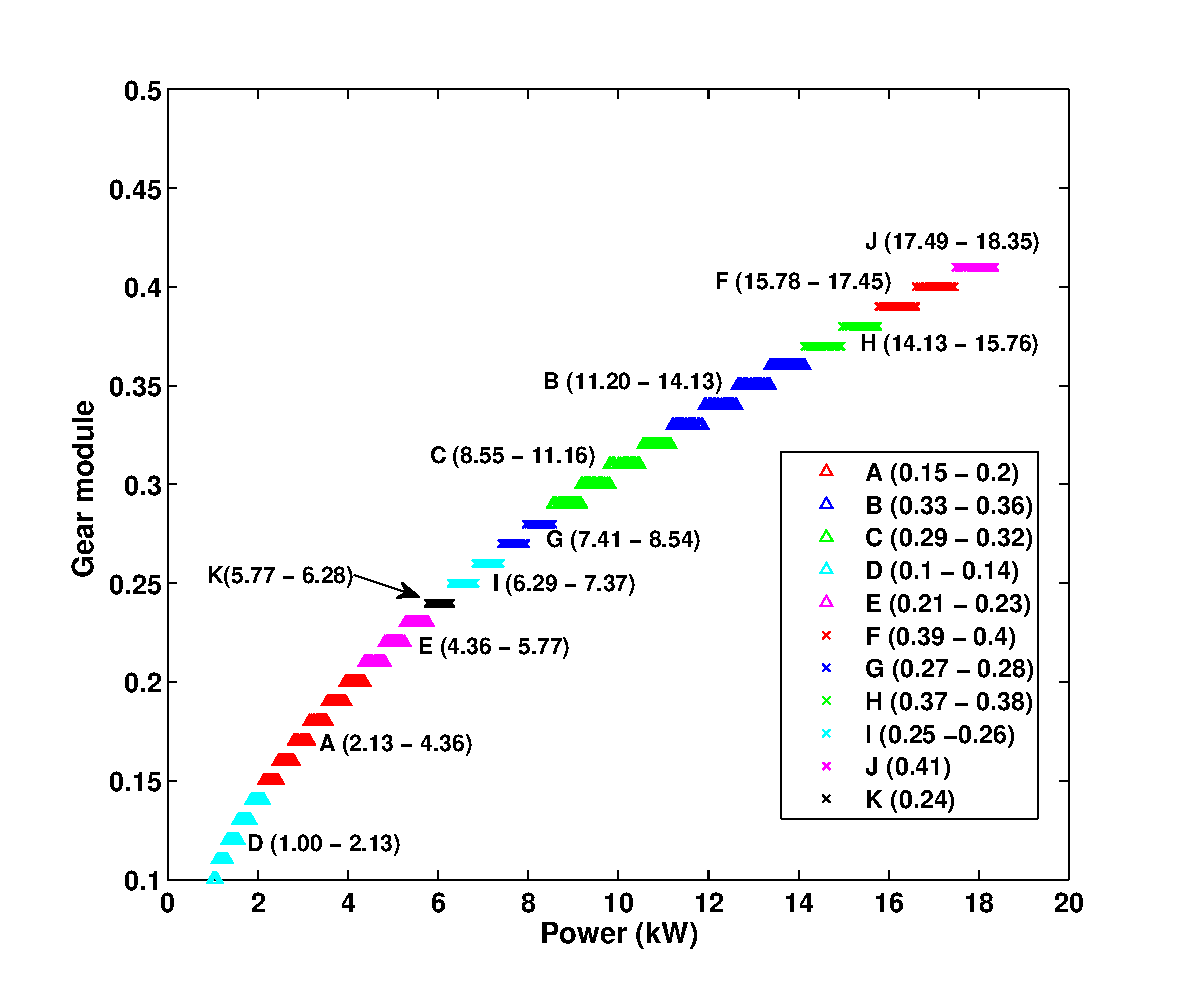
\includegraphics[width=100mm, height=80mm]{dia/gt11pVsm.eps}
 \caption{Power Vs. module characteristics of the pareto-front}
 \label{gt11pVsm}
\end{center}\end{figure}


\begin{table}[!ht]
  \centering
  \begin{tabular}{|c|c|c|c|c|c|}
    \hline
    \multirow{2}{*}{A}   & ($p$) &  ($t_8$) &  ($t_9$)  & ($m$) & ($t_7$)\\
    & 0.9979  & 0.0404  & 0.0283 & 0.0261 & 0.0178  \\
    \hline
    \multirow{2}{*}{B}   & ($p$) &  ($t_8$) &  ($m$)  & ($t_9$) & ($t_7$)\\
    & 0.9996 & 0.0154 & 0.0125 & 0.0106 &  0.0078 \\
    \hline
    \multirow{2}{*}{C} & ($p$) & ($t_8$) & ($t_9$) &  ($m$) & ($t_7$) \\
    & 0.9990 & 0.0258 & 0.0191 & 0.0138 & 0.0130 \\
    \hline
    \multirow{4}{*}{D} & ($p$) & ($t_8$) & ($t_9$) &  ($t_7$) & ($m$) \\
    & 0.9916 & 0.0793 & 0.0627 & 0.03979 & 0.03754 \\ 
    \cline{2-6}
    & ($t_8$) & ($t_9$) & ($t_7$) &  ($t_4$) & ($t_5$) \\
    & -0.6456 & -0.4667 & -0.3213 & -0.2941 & -0.2625 \\
    \hline
    \multirow{2}{*}{E} & ($p$) & ($t_8$) & ($t_9$) &  ($t_7$) & ($t_5$) \\
    & 0.9939 & 0.0706 & 0.0503 & 0.0378 & 0.0288 \\ 
    \hline
    \multirow{2}{*}{F} & ($p$) & ($t_8$) & ($t_9$) &  ($t_7$) & ($t_4$) \\
    & 0.9982 & 0.0388 & 0.0275 & 0.0190 & 0.0175 \\ 
    \hline
    \multirow{2}{*}{G} & ($p$) & ($t_8$) & ($t_9$) &  ($t_7$) & ($t_6$) \\
    & 0.9924 & 0.0799 & 0.0572 & 0.0403 & 0.0335 \\ 
    \hline
    \multirow{2}{*}{H} & ($p$) & ($t_8$) & ($t_9$) &  ($t_7$) & ($t_5$) \\
    & 0.9975 & 0.0470 & 0.0314 & 0.0227 & 0.0193 \\ 
    \hline
    \multirow{2}{*}{I} & ($p$) & ($t_8$) & ($t_9$) &  ($t_7$) & ($t_4$) \\
    & 0.986 & 0.1056 & 0.0796 & 0.0536 & 0.0486 \\ 
    \hline
    \multirow{2}{*}{J} & ($p$) & ($t_8$) & ($t_9$) &  ($t_7$) & ($t_4$) \\
    & 0.9779 & 0.1326 & 0.1002 & 0.0655 & 0.0621 \\ 
    \hline
    \multirow{2}{*}{K} & ($p$) & ($t_8$) & ($t_9$) &  ($t_7$) & ($t_4$) \\
    & 0.852 & 0.3395 & 0.2502 & 0.1748 & 0.1416 \\ 
    \hline
  \end{tabular}
  \caption{First principal components of the pareto-front of the fixed lay-out gear-box design problem}
  \label{first2GTPCs}
\end{table}



\begin{figure}[ht]\begin{center}
 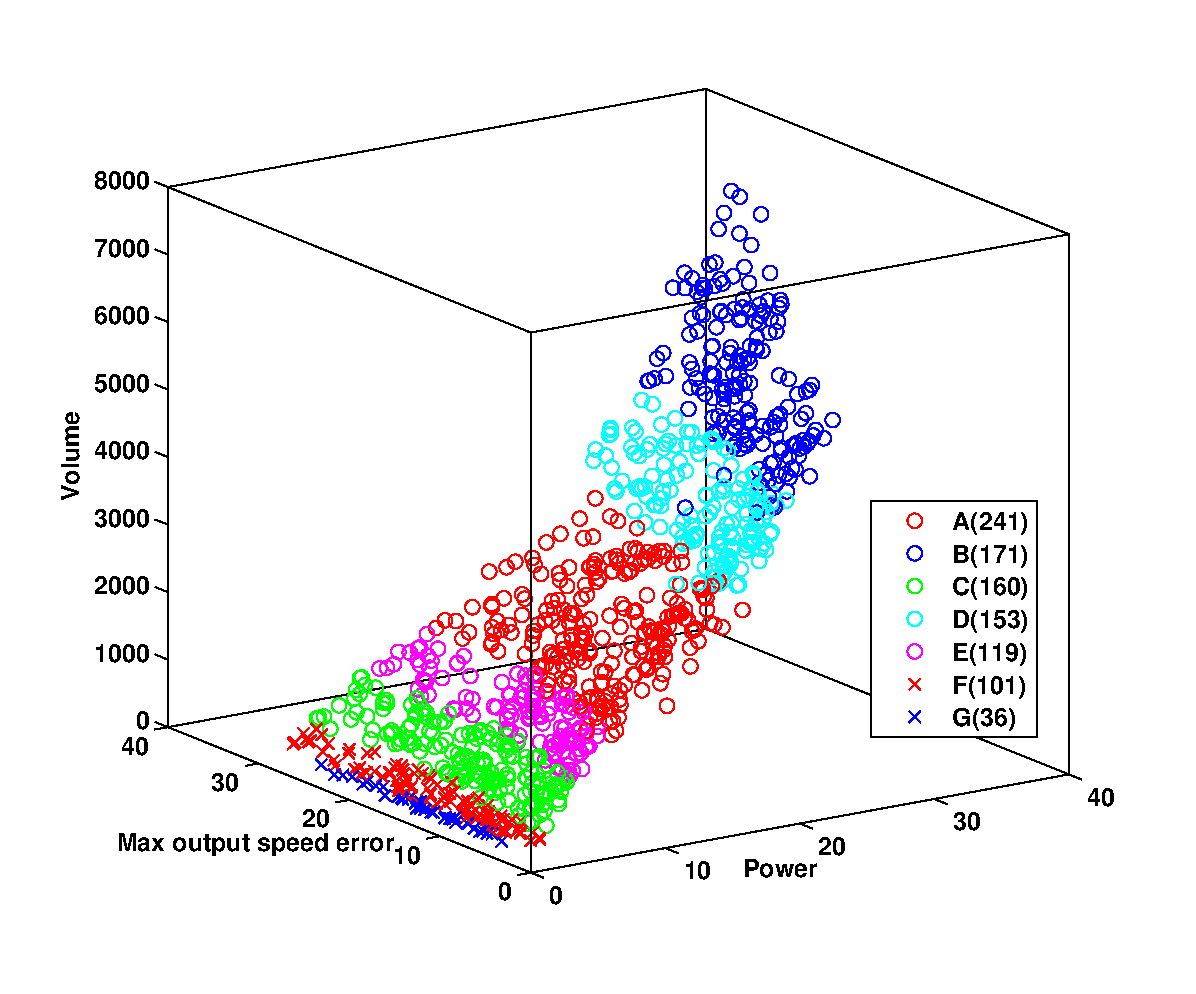
\includegraphics[width=100mm, height=80mm]{dia/gtvopareto2.eps}
 \caption{Clusters for the 29-variable problem}
 \label{gtvClusters}
\end{center}\end{figure}


\begin{figure}[ht]\begin{center}
 \subfloat[Isomap Residual Variance for clusters A, C and E.]{
 \label{gt11rv} 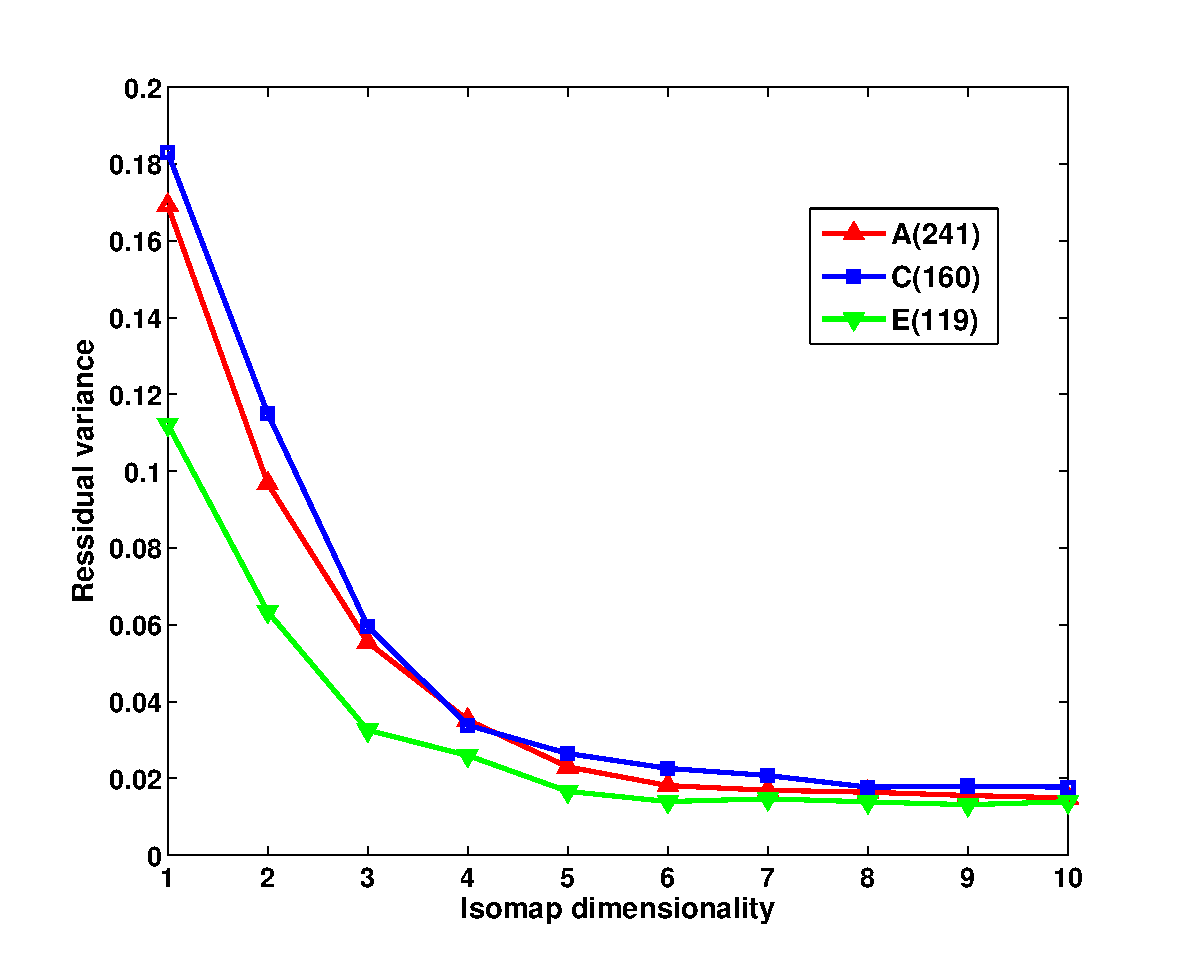
\includegraphics[width=62mm, height=52mm]{dia/gtvcrv1.eps}}
 \subfloat[Isomap Residual variances for clusters B, C, E and F]{
 \label{gt11ev} 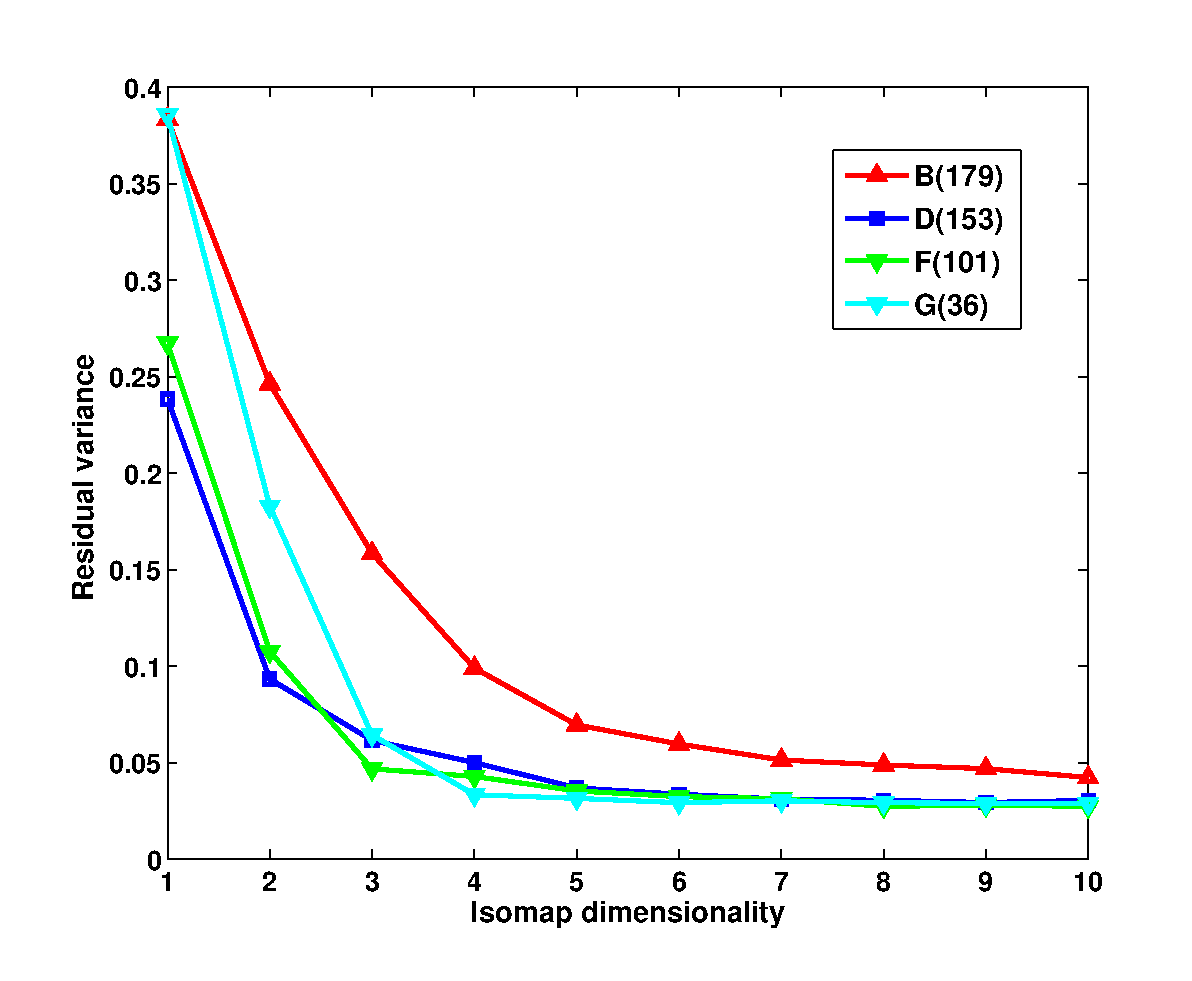
\includegraphics[width=62mm, height=52mm]{dia/gtvcrv2.eps}}
 \caption{Isomap residual variances for clusters for the variable gear teeth problem}
 \label{gtvClustersRV}
\end{center}\end{figure}

\begin{figure}[ht]\begin{center}
 \subfloat[Cumulative explained variance for clusters A, B, C and D]{
 \label{gt11rv} 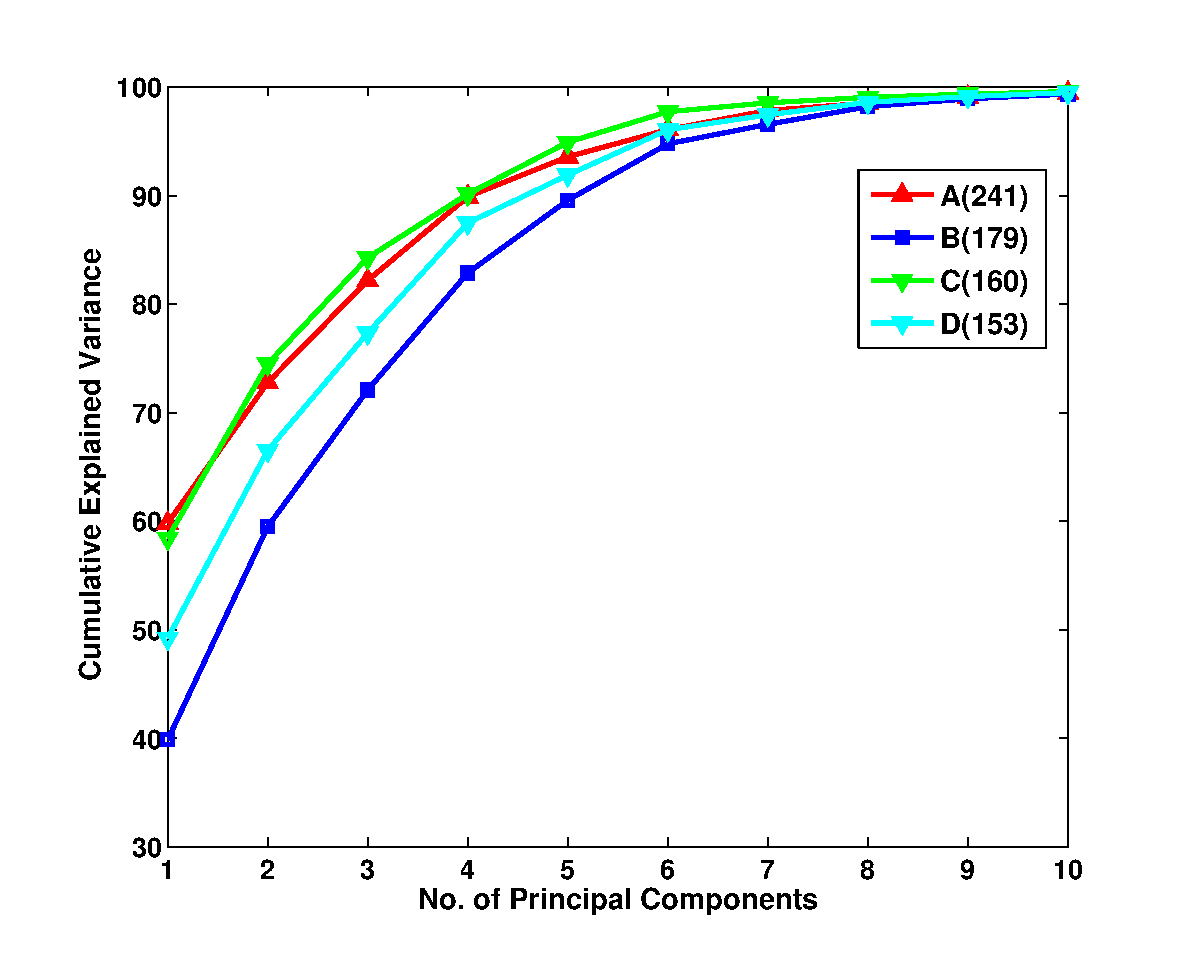
\includegraphics[width=62mm, height=52mm]{dia/gtvicev1.eps}}
 \subfloat[Isomap Residual variances for clusters E, F and G]{
 \label{gt11ev} 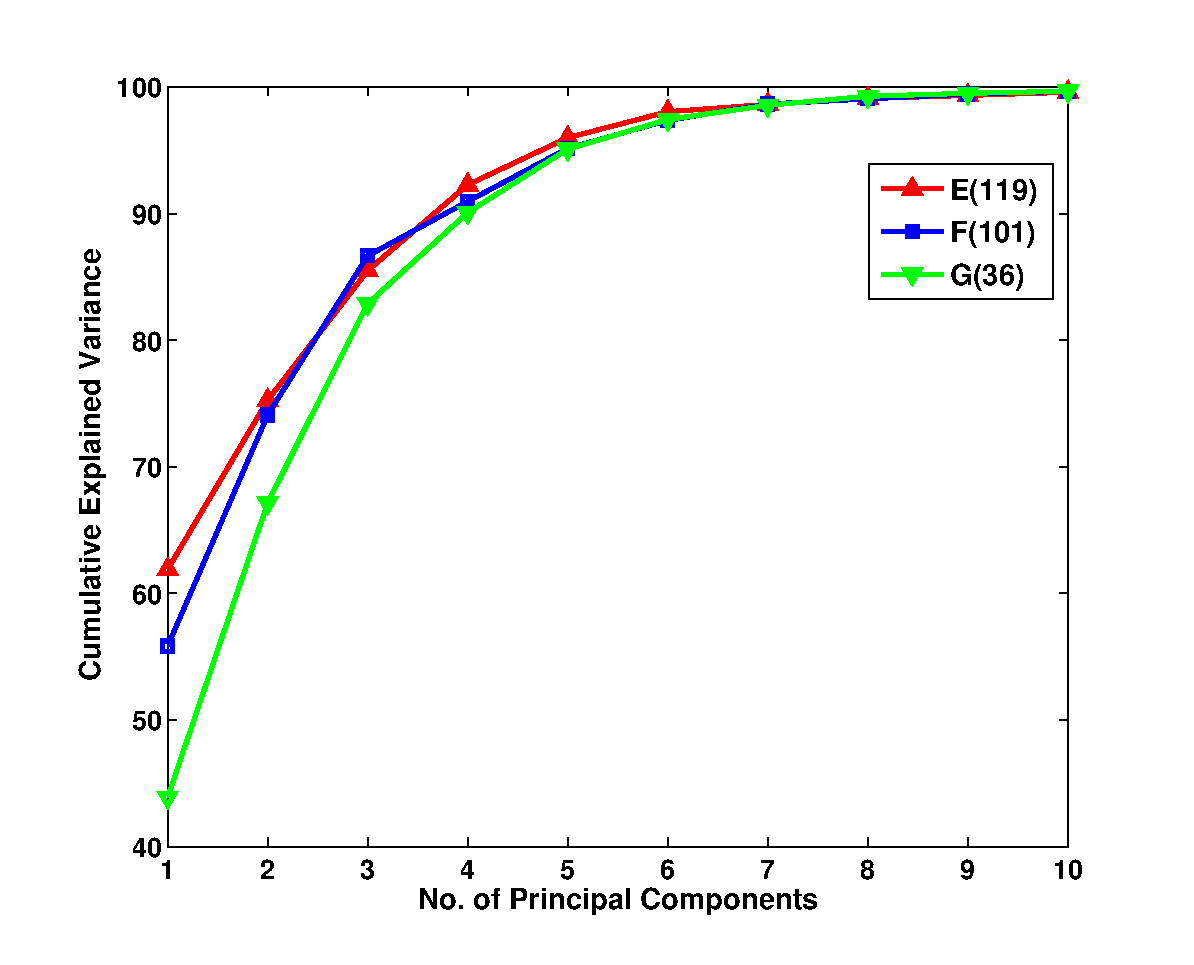
\includegraphics[width=62mm, height=52mm]{dia/gtvicev2.eps}}
 \caption{Cumulative PCA explained variance for 29 variable problem}
 \label{gtvClustersEV}
\end{center}\end{figure}



\begin{figure}[ht]\begin{center}
 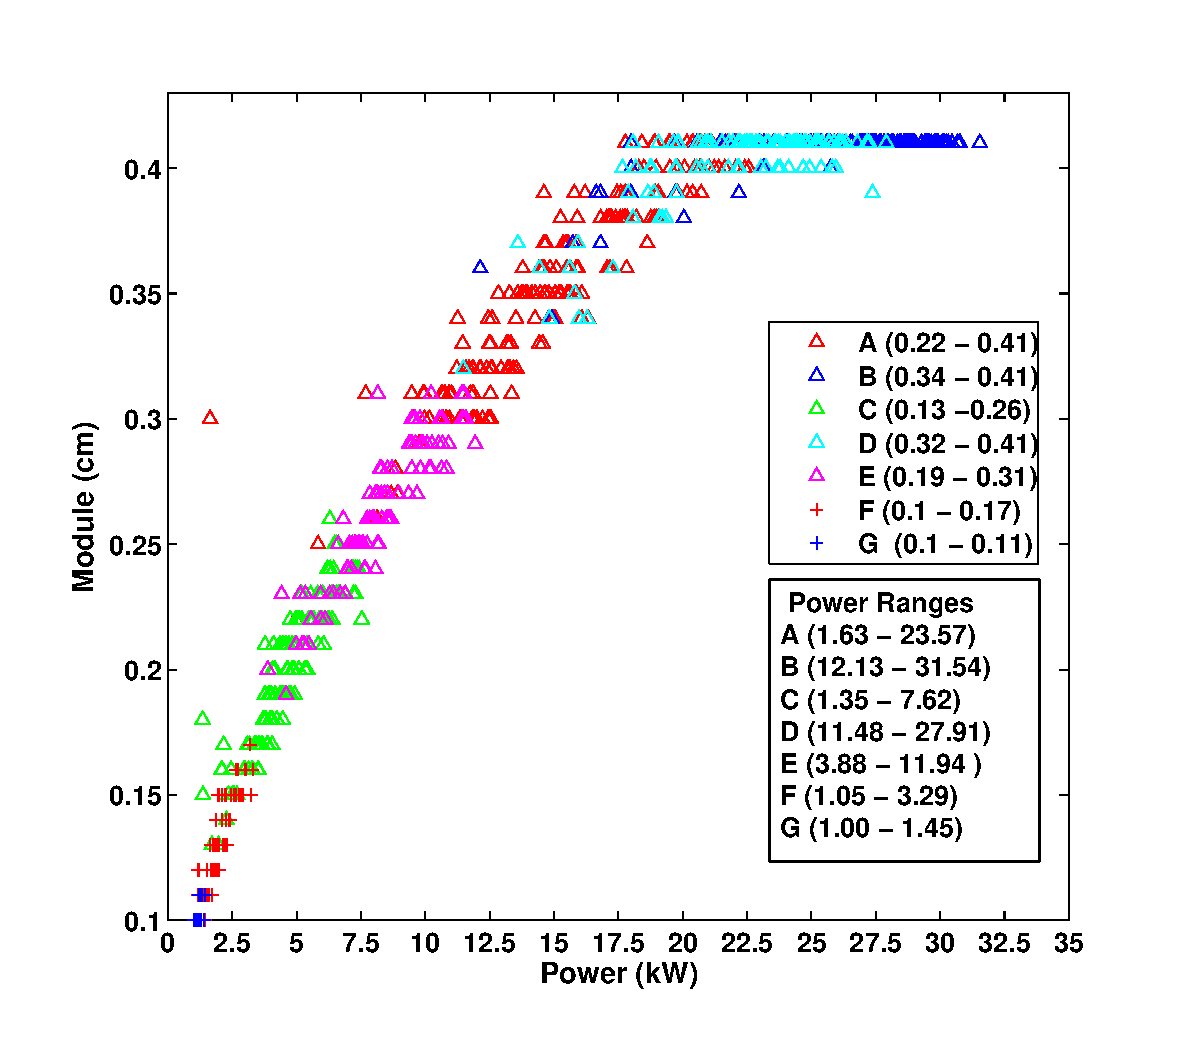
\includegraphics[width=100mm, height=80mm]{dia/gtvpVsm.eps}
 \caption{Power Vs. module characteristics of the pareto-front for variable gear teeth problem}
 \label{gtvpVsm}
\end{center}\end{figure}
   


\begin{table}[!ht]
  \centering
  \begin{tabular}{|c|c|c|c|c|c|c|c|c|c|c|c|c|}
    \hline
    \multirow{2}{*}{A} & First PC & $n_{8}$ & $n_{9}$ & $n_{12}$ & $n_{6}$ & $n_{7}$ & $n_{11}$ & $\dots$ & \cellcolor{magenta} $ n_{16}$ & \cellcolor{orange} $n_{18}$ & \cellcolor{green} $n_{15}$ & \cellcolor{cyan} $n_{17}$ \\ \cline{2-13}
    & Second PC & $n_{11}$ & $n_{13}$ & $n_{10}$ & $n_{12}$ & $n_{5}$ & $n_{6}$ & $\dots$ & \cellcolor{cyan} $n_{17}$ & \cellcolor{magenta} $n_{16}$ & \cellcolor{green} $n_{15}$ & \cellcolor{orange} $n_{18}$ \\
    \hline
    \cline{1-13}
    \multirow{2}{*}{B}& First PC & $n_{12}$ & $n_{8}$ & $n_{11}$ & $n_{6}$ & $n_{5}$ & $n_{9}$ & $\dots$ &  \cellcolor{cyan} $n_{17}$ & \cellcolor{green} $n_{15}$ & \cellcolor{magenta} $n_{16}$ & \cellcolor{orange} $n_{18}$ \\ 
    \cline{2-13}
    & Second PC & $n_{11}$ & $n_{10}$ & $n_{8}$ & $n_{12}$ & $n_{6}$ & $n_{13}$ & $\dots$ &  \cellcolor{green} $n_{15}$ & \cellcolor{cyan} $n_{17}$ & \cellcolor{magenta}$n_{16}$ & \cellcolor{orange} $n_{18}$ \\ 
    \hline
    \cline{1-13}
    \multirow{2}{*}{C}& First PC & $n_{11}$ & $n_{7}$ & $n_{10}$ & $n_{6}$ & $n_{9}$ & $n_{5}$ & $\dots$ &  \cellcolor{cyan} $n_{17}$ & \cellcolor{orange} $n_{18}$ & \cellcolor{green}$n_{15}$ & \cellcolor{magenta} $n_{16}$ \\ 
    \cline{2-13}
    & Second PC & $n_{12}$ & $n_{6}$ & $n_{8}$ & $n_{11}$ & $n_{9}$ & $n_{10}$ & $\dots$ &  \cellcolor{green} $n_{15}$ & \cellcolor{magenta} $n_{16}$ & \cellcolor{orange}$n_{18}$ & \cellcolor{cyan} $n_{17}$ \\ 
    \hline
    \cline{1-13}
    \multirow{2}{*}{D}& First PC & $n_{9}$ & $n_{8}$ & $n_{10}$ & $n_{5}$ & $n_{12}$ & $n_{7}$ & $\dots$ &  \cellcolor{green} $n_{15}$ & \cellcolor{magenta} $n_{16}$ & \cellcolor{cyan} $n_{17}$ & \cellcolor{orange} $n_{18}$ \\ 
    \cline{2-13}
    & Second PC & $n_{10}$ & $n_{12}$ & $n_{11}$ & $n_{7}$ & $n_{6}$ & $n_{8}$ & $\dots$ &  \cellcolor{cyan} $n_{17}$ & \cellcolor{green} $n_{15}$ & \cellcolor{orange} $n_{18}$ & \cellcolor{magenta} $n_{16}$ \\ 
    \hline
    \cline{1-13}
    \multirow{2}{*}{E}& First PC & $n_{8}$ & $n_{9}$ & $n_{12}$ & $n_{6}$ & $n_{11}$ & $n_{13}$ & $\dots$ &  \cellcolor{orange} $n_{18}$ & \cellcolor{cyan} $n_{17}$ & \cellcolor{green}$n_{15}$ & \cellcolor{magenta} $n_{16}$ \\ 
    \cline{2-13}
    & Second PC & $n_{9}$ & $n_{8}$ & $n_{12}$ & $n_{7}$ & $n_{10}$ & $n_{4}$ & $\dots$ &  \cellcolor{magenta} $n_{16}$ & \cellcolor{green} $n_{15}$ & \cellcolor{cyan}$n_{17}$ & \cellcolor{orange} $n_{18}$ \\ 
    \hline
    \cline{1-13}
    \multirow{2}{*}{F}& First PC & $n_{11}$ & $n_{9}$ & $n_{6}$ & $n_{8}$ & $n_{5}$ & $n_{7}$ & $\dots$ &  \cellcolor{magenta} $n_{16}$ & \cellcolor{green} $n_{15}$ & \cellcolor{orange}$n_{18}$ & \cellcolor{cyan} $n_{17}$ \\ 
    \cline{2-13}
    & Second PC & $n_{8}$ & $n_{6}$ & $n_{7}$ & $n_{9}$ & $n_{11}$ & $n_{5}$ & $\dots$ &  \cellcolor{magenta} $n_{16}$ & \cellcolor{orange} $n_{18}$ & \cellcolor{cyan}$n_{17}$ & \cellcolor{green} $n_{15}$ \\ 
    \hline
    \cline{1-13}
    \multirow{2}{*}{F}& First PC & $n_{11}$ & $n_{13}$ & $n_{6}$ & $n_{7}$ & $n_{9}$ & $n_{8}$ & $\dots$ &  \cellcolor{cyan} $n_{17}$ & \cellcolor{green} $n_{15}$ & \cellcolor{magenta}$n_{16}$ & \cellcolor{orange} $n_{18}$ \\ 
    \cline{2-13}
    & Second PC & $n_{12}$ & $n_{4}$ & $n_{8}$ & $n_{10}$ & $n_{9}$ & $n_{11}$ & $\dots$ &  \cellcolor{cyan} $n_{17}$ & \cellcolor{magenta} $n_{16}$ & \cellcolor{green}$n_{15}$ & \cellcolor{orange} $n_{18}$ \\ 
    \hline
  \end{tabular}
  \caption{Ranking of gear teeth variables on the basis of absolute weights in principal components.}
  \label{first2gtvnt}
\end{table}


% \multirow{2}{*}{}& First PC & $n_{}$ & $n_{}$ & $n_{}$ & $n_{}$ & $n_{}$ & $n_{}$ & $\dots$ &  \cellcolor{} $n_{}$ & \cellcolor{} $n_{}$ & \cellcolor{}$n_{}$ & \cellcolor{} $n_{}$ \\ 
%\cline{2-13}
% & Second PC & $n_{}$ & $n_{}$ & $n_{}$ & $n_{}$ & $n_{}$ & $n_{}$ & $\dots$ &  \cellcolor{} $n_{}$ & \cellcolor{} $n_{}$ & \cellcolor{}$n_{}$ & \cellcolor{} $n_{}$ \\ 
%\hline

\message{ !name(GTproblem.tex) !offset(-455) }
 